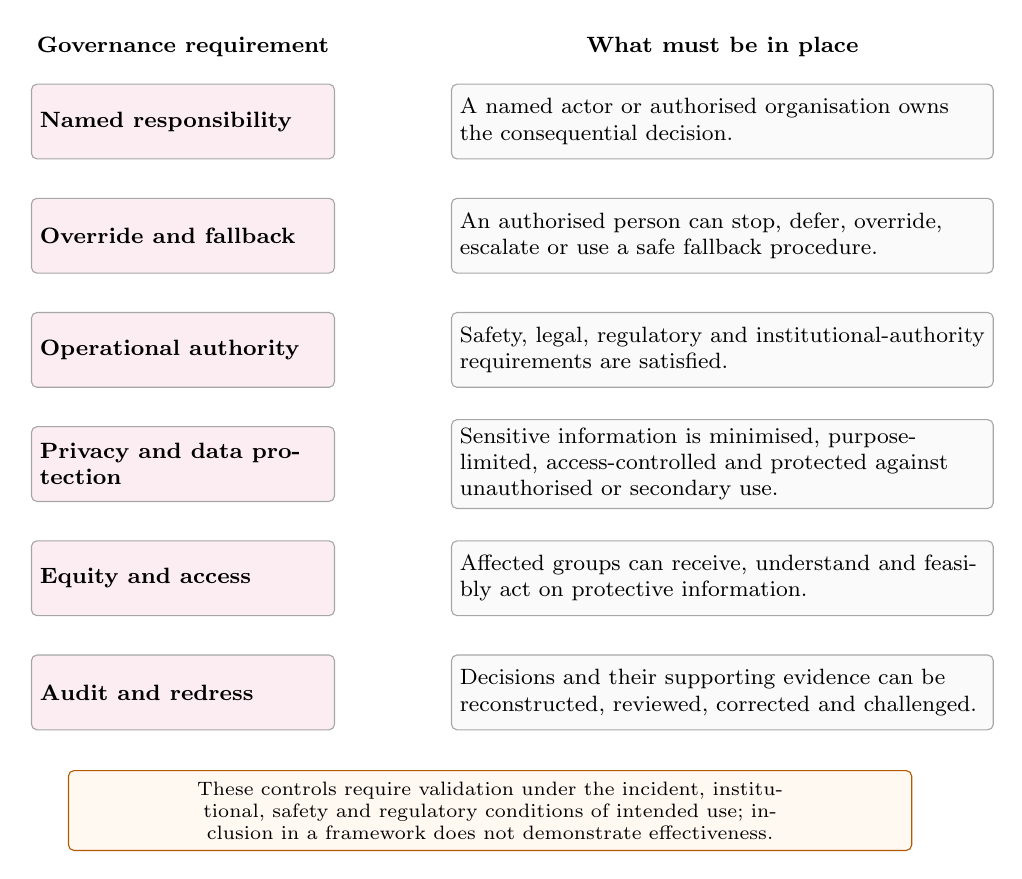
\begin{tikzpicture}[
row/.style={draw=black!35,rounded corners=2pt,minimum height=9.5mm,inner sep=3pt,font=\footnotesize,text=black},
req/.style={row,fill=purple!7,align=left,text width=0.30\linewidth,font=\bfseries\footnotesize},
meaning/.style={row,fill=black!2,align=left,text width=0.55\linewidth},
head/.style={font=\bfseries\footnotesize,text=black}
]
\node[head] at (2.1,0.45) {Governance requirement};
\node[head] at (8.95,0.45) {What must be in place};
\node[req] (r1) at (2.1,-0.5) {Named responsibility};
\node[meaning] (m1) at (8.95,-0.5) {A named actor or authorised organisation owns the consequential decision.};
\node[req] (r2) at (2.1,-1.95) {Override and fallback};
\node[meaning] (m2) at (8.95,-1.95) {An authorised person can stop, defer, override, escalate or use a safe fallback procedure.};
\node[req] (r3) at (2.1,-3.40) {Operational authority};
\node[meaning] (m3) at (8.95,-3.40) {Safety, legal, regulatory and institutional-authority requirements are satisfied.};
\node[req] (r4) at (2.1,-4.85) {Privacy and data protection};
\node[meaning] (m4) at (8.95,-4.85) {Sensitive information is minimised, purpose-limited, access-controlled and protected against unauthorised or secondary use.};
\node[req] (r5) at (2.1,-6.30) {Equity and access};
\node[meaning] (m5) at (8.95,-6.30) {Affected groups can receive, understand and feasibly act on protective information.};
\node[req] (r6) at (2.1,-7.75) {Audit and redress};
\node[meaning] (m6) at (8.95,-7.75) {Decisions and their supporting evidence can be reconstructed, reviewed, corrected and challenged.};
\node[draw=orange!70!black,fill=orange!5,rounded corners=2pt,align=center,text width=0.86\linewidth,inner sep=4pt,font=\scriptsize,text=black] at (6.0,-9.25)
{These controls require validation under the incident, institutional, safety and regulatory conditions of intended use; inclusion in a framework does not demonstrate effectiveness.};
\end{tikzpicture}
